\begin{table*}[t]
\caption{Accumulated rewards split by origin per setting. Evaluation was done after every episode of training and the best result is shown. The best performance on each sub-task is highlighted per experiment.}
\label{tab:experiments}
\vskip 0.15in
\begin{center}
\begin{small}
\begin{sc}
\begin{tabular}{lcccccr}
\toprule
Experiment & Algorithm & ESS & FDR & TCL & Discomfort & Total \\
\midrule
\multirow{4}{*}{Initial Setting} 
    & Idle      & 0.00   & -3173.56 & -9887.61  & -5912.63  & -21746.74 \\
    & Random    & -87.56 & -3112.28 & -33017.25 & -8562.27  & -47552.30 \\
    & Threshold & \textbf{633.24} & -3068.56 & \textbf{-10988.57} & \textbf{-1106.55}  & \textbf{-17303.38} \\
    & PPO       & 0.00   & \textbf{-3038.80} & -10749.44 & -1423.62  & -17984.79 \\
    & SAC       & -82.24 & -3063.11 & -10036.19 & -4958.21  & -20912.68 \\
\midrule
\multirow{4}{*}{Stacked Carbon Intensity}
    & Idle      & 0.00   & -3173.56 & -9887.61  & -5912.63  & -21746.74 \\
    & Random    & -87.56 & -3112.28 & -33017.25 & -8562.27  & -47552.30 \\
    & Threshold & \textbf{633.24} & -3068.56 & -10988.57 & -1106.55  &  \textbf{-17303.38} \\
    & PPO       & 0.00   & \textbf{-3017.24} & \textbf{-10810.46} &  \textbf{-1180.09}  & -17780.73 \\
    & SAC       & -18.01 & -3077.25 & -10226.50 & -3403.34  & -19498.02 \\
\midrule
\multirow{4}{*}{Eased Exploration}
    & Idle      & 0.00   & -3173.56 & -9887.61  & -5912.63 & -21746.74 \\
    & Random    & -90.93 & -3112.33 & -32818.01 & -9205.60  & -47999.80 \\
    & Threshold & \textbf{633.24} & -3056.79 & \textbf{-10988.57} & \textbf{-1106.55} & \textbf{-17290.67} \\
    & PPO       & 0.00   & -3034.17 & -10055.01  & -5072.91 & -20933.18  \\
    & SAC       & 495.07 & \textbf{-2952.68} & -12908.10 & -4582.26 & -22720.31  \\
\midrule
\multirow{4}{*}{Terminal Reward} 
    & Idle      & 0.00   & -3173.56 & -9887.61  & -5912.63  & -21746.74 \\
    & Random    & -87.56 & -3112.28 & -33017.25 & -8562.27  & -47552.30 \\
    & Threshold & \textbf{633.24} & \textbf{-3068.56} & \textbf{-10988.57} & \textbf{-1106.55}  & \textbf{-17303.38} \\
    & PPO       & 362.88 & -3125.46 & -10759.23 & -1587.45  & -17881.28 \\
    & SAC       & -92.20  & -3123.76 & -13036.89 & -3371.14  & -22395.99 \\
\bottomrule
\end{tabular}
\end{sc}
\end{small}
\end{center}
\vskip -0.1in
\end{table*}

As non-learning baselines an idle policy, which would always return zero actions, whose cumulative reward in the first episode is shown in \cref{fig:reward_idle}, a random policy, and a thresholding policy, see \cref{sec:thresholding_baseline}, were implemented.

\begin{figure}[H]
    \centering
    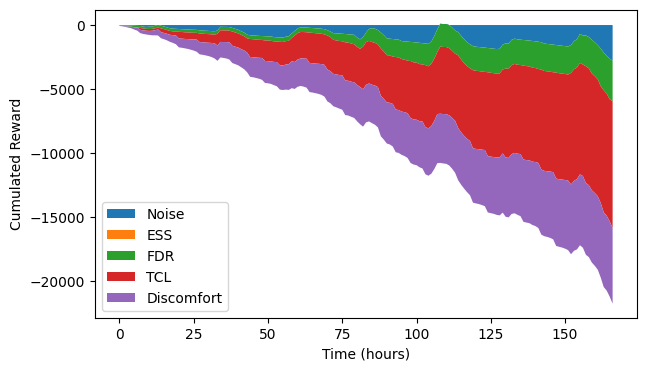
\includegraphics[width=0.45\textwidth]{figures/idle_reward.png}
    \caption{Cumulative reward for the idle policy.}
    \label{fig:reward_idle}
\end{figure}

As learning agents, Soft Actor Critic (SAC) \cite{Haarnoja.04.01.2018} and Proximal Policy Optimization (PPO) \cite{Schulman.20.07.2017} were chosen. Both implementations were taken from \textit{stable baselines 3} \cite{AntoninRaffin.2021}, for more details see \cref{sec:sac} and \cref{sec:ppo}.
\par
Since RL algorithms are known to be sample inefficient \cite{rlblogpost}, the environment was initially restricted to a single episode in an effort to accelerate convergence. The training curve is shown in \cref{fig:training_curve} and all results in \cref{tab:experiments}. Rewards were split by origin, as in \cref{sec:split_reward}, to allow evaluation by task. The results were convergent but not satisfactory, since the agents did not outperform the thresholding baseline. The agents were unable to utilize the ESS effectively, while TCL and FDR actions were also far from optimal.
\begin{figure}[H]
    \centering
    \setlength{\abovecaptionskip}{0pt}
    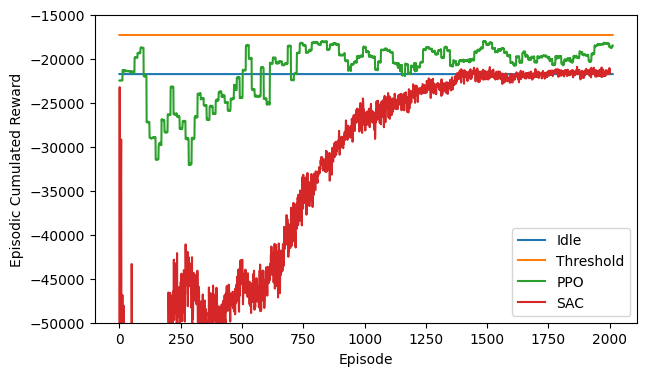
\includegraphics[width=0.45\textwidth]{figures/training_curve.png}
    \caption{Training curve replaying a single episode.}
    \label{fig:training_curve}
\end{figure}
To increase the learnability of the environment three variations were tested. Additional details about them can be found in \cref{sec:training_procedure}.


\subsection{Stacked Carbon Intensity}
To effectively act on any sub-task, the current carbon intensity has to be evaluated against the expected future. If the agents would fail to recognize low carbon intensity, their poor performance across sub-tasks would be explained.
\par
To ease this task the carbon intensity observable was stacked into the future.  While this improved the overall performance marginally, the primary issue remained.


\subsection{Eased Exploration}
The action space in the given setting is continuous and high dimensional, due to the dependence on $H$. In combination with the stochasticity of FDR control and the noisy reward, discovering effective action sequences is challenging.
\par
To shrink the action space, the FDR control was collapsed into a scalar. Moreover, actions were discretised for PPO and the agents were trained separately for each sub-task. The FDR control was also changed to deterministically control the consumption. This assumes that the optimal policy is invariant to $U_e$ as long as the sum is maintained and that $\beta = \infty$. In addition, the RSA and household energy demand were removed from the observables and reward calculation.
\par
The separate training enabled SAC to utilize the ESS effectively, while performance on the other sub-tasks remained poor. PPO performed significantly worse, which is probably due to the discretisation of the action space.


\subsection{Terminal Reward}
Another challenge of the setting is the reward structure for charging the ESS, expediting the FDR and heating or cooling the TCL. An effective policy requires those actions, but they are always penalized immediately, while the associated reward occurs delayed and only if the respective counter action is performed at a higher carbon intensity.
\par
To remove the temporal reward-action tie, the reward was transferred to an accumulating observable and only actuated in the terminal state, which should encourage the agent to evaluate the entire trajectory of an episode holistically. This enabled PPO to effectively utilize the ESS, however the performance on all other sub-tasks worsened. Moreover, SAC performed significantly worse across sub-tasks.